\documentclass[../Main/Main.tex]{subfiles}

\begin{document}
Antes de poder continuar con la construcción y definir por completo al modelo \textit{bpwpm}, se debe hacer una pausa y estudiar los fundamentos de la escuela bayesiana de la estadística. Esto pues el algoritmo asociado al modelo recae en un método fundamental de la disciplina: el muestreador de Gibbs.

\section{Fundamentos de la estadística bayesiana}
Dado el problema de describir fenómenos bajo incertidumbre, existen dos escuelas dominantes de la estadística: la frecuentista y la bayesiana. %La primera, aunque útil, no está del todo axiomatizada y en ocasiones termina derivando en colecciones de algoritmos. 
La escuela bayesiana, nombrada así en honor a Thomas Bayes (1702 - 1761), enfatiza el componente \textit{probabilista} del proceso inferencial, desarrollando un paradigma completo para la inferencia y la toma de decisiones bajo incertidumbre. Asimismo, la estadistica bayesiana está axiomatizada bajo la \textit{teoría de la decisión}. Esta teoría formaliza conceptos como la coherencia entre preferencias y utilidad, sobre los que desarrolla un marco metodológic, \citet{bernardo2001bayesian} y \citet{mendoza2011estadistica}.

Esta metodología, además de proveer técnicas concretas para resolver problemas, también formaliza en una forma de pensar sobre la probabilidad como una \textit{medida racional para cuantificar la incertidumbre}. Este paradigma es el que más corresponde con el sentido que usualmente se le da a la palabra. La inferencia o predicción sobre eventos, se realiza mediante una \textit{actualización} de la información que se tiene bajo la luz de nueva evidencia, modificando así la medida de incertidumbre. El mecanismo que permite realizar este proceso de actualización es el teorema de Bayes. De manera informal el teorema \eqref{ec:BayesInformal} explica que dado un evento $E$ bajo condiciones $C$, la probabilidad \textit{posterior} de ocurrencia del evento, será proporcional a la probabilidad \textit{previa} que se tiene sobre este, ponderado por la probabilidad de ocurrencia de las condiciones presentes. \\ %En menos palabras, el teorema de Bayes está  actualizando la probabilidad de ocurrencia de un evento ponderando esta probabilidad por la información que se tiene sobre el. 

\begin{theorem} El teorema de Bayes (informal):
\begin{align}
P(E|C) \propto P(C|E)P(E) \label{ec:BayesInformal}
\end{align}
\end{theorem}
\vspace*{-.7cm}
Donde, el término central $P(C|E)$ es una medida descriptiva de las condiciones (usualmente datos), $P(E)$ es la probabilidad previa (\textit{a priori}) que se tiene del evento $E$ y $P(E|C)$ es la probabilidad posterior del evento (actualizada).

En un contexto de estadistica paramétrica más formal, los eventos por estudiar $E$ se abstraen en una serie de parámetros $\theta$ que usualmente son desconocidos. Asimismo las condiciones $C$ quedan resumidas en datos observados $\mathbf{X}$ que son interpretados como \textit{evidencia}. 
Bajo este paradigma antes de poder hacer cualquier intento de inferencia sobre $\theta$, se debe especificar el \textit{modelo probablistico} que se asume describe el fenómeno observado, pues es a través de este modelo que se da una medida concreta para cuantificar la incertidumbre. Asimismo, se tienen ciertas creencias, hipótesis u conocimiento previo, \textit{a priori}, sobre los parámetros $\theta$, los cuales se representan por una medida de probabilidad $\pi(\theta)$. Segundo, se tienen datos $\mathbf{X}$ a los que se asigna un modelo de probabilidad en función de los parámetros $\pi(\mathbf{X}|\theta)$, a la que se le conoce como \textit{verosimilitud} \autocite{bernardo2003bayesian}.\\
\begin{theorem}
El teorema de Bayes:
\begin{align} 
	\pi(\theta|\mathbf{X}) \propto \pi(\mathbf{X}|\theta)\,\pi(\theta)\label{ec:BayesProporcional}
\end{align}
\end{theorem}
\vspace*{-.7cm}
Habiendo especificado el modelo, el teorema de Bayes \eqref{ec:BayesProporcional} describe el proceso de actualización de conocimiento sobre los parámetros $\theta$. La idea es que este proceso de actualización sea, de la misma forma, un \textit{proceso de aprendizaje}, en el cual los parámetros capturen la información contenida en los datos.

Bajo el paradigma frecuentista, se adopta un enfoque diferente para el  aprendizaje. Se asume que no hay incertidumbre inherente en los parámetros dado los datos por lo que simplemente son desconocidos y estos  se deben de estimar. El mecanismo que permite su estimación, usualmente consiste en plantear una función objetivo y optimizarla. Por ejemplo, si se escoge la verosimilitud $\pi(\mathbf{X}|\theta)$, se busca dar un estimador $\hat{\theta}$ que la maximice, pues equivaldría a encontrar los parámetros que hagan más \textit{posibles} los datos bajo el modelo planteado. Si por el contrario, es escoge una función como la suma de residuales cuadrados (RSS por sus siglas en inglés) de los modelos ANOVA, se busca un estimador $\hat{\theta}$ que minimice los residuales, así, el modelo logra capturar toda la variabilidad posible contenida en los datos. Independientemente del paradigma estadístico que se escoja, siempre es importante la validación del modelo y de sus supuestos. No obstante, tanto la teoría bayesiana como la frecuentista han resultado de infinita utilidad en la práctica y el avance de la estadística y ciencia en general.

Una de las dificultades que surgen en la estadística bayesiana, es que la obtención de resultados analíticos cerrados es difícil, sino imposible, una vez que los modelos se complican. Para ejemplificar, en los teoremas anteriores, se ha usado el argumento de proporcionalidad $\propto$. Esto pues, para que se de la igualdad, el lado derecho de la ecuación \eqref{ec:BayesProporcional} se debe dividir entre la probabilidad total de la ocurrencia de los datos bajo el modelo planteado: $$\pi(\mathbf{X}) = \int \pi(X|\tilde{\theta})\,\pi(\tilde{\theta})\,d\tilde{\theta},$$ el cual usualmente es difícil de calcular analíticamente. A este término se le conoce como \textit{constante de proporcionalidad} y su función es la de reescalar la expresión del lado derecho de la ecuación \eqref{ec:BayesProporcional} para que en realidad se tenga una distribución en el izquierdo. Usualmente para evitar estas complicaciones, se escogen \textit{distribuciones conjugadas}, para que tanto la distribución a priori como la posterior pertenezcan a la misma familia.\footnote{En el apéndice \ref{ap:DistrosConjugadas} se detallan las distribuciones conjugadas y se realiza más a fondo la derivación de los resultados de este trabajo.} Sin embargo, con los avances en el poder computacional disponible y técnicas numéricas para resolver integrales \autocite{robert2004monte}, se han desarrollado muchos métodos para aplicar el proceso de aprendizaje independientemente de que tan complejo sea el modelo. Muchos de estos métodos recaen en el uso de algoritmos numéricos de simulación estocástica llamados \emph{cadenas de Markov Monte Carlo} \footnote{MCMC por sus siglas en inglés.} como lo es el muestreador Gibbs a presentarse en la sección \ref{sec:GibbsSampler}. 

\subsubsection{Estimadores Bayesianos}
Una vez realizado el proceso de actualización, se cuenta con una distribución posterior de probabilidad para los parámetros de interés.\footnote{Es común tener en la práctica, no es la distribución analítica, sino una muestra de ella debido al proceso numérico usado para llegar a ella.} No obstante, por practicaldiad y utilidad, en ocasiones se busca dar un \textit{estimador puntual} de los parámetros. La teoría de la decisión dicta que para medir la deseabilidad de escoger cierto parámetro en particular, se debe definir una función de perdida ($L$) o utilidad que optimice esta elección. Particularmente, las funciones de perdida logran medir las consecuencias incurridas al tomar $\hat{\theta}$ como el valor puntual del parámetro; lo hacen, penalizando la distancia entre el \emph{valor real} $\theta$ y su estimador puntual $\hat{\theta}$. Por lo tanto y sin entrar mucho en los detalles técnicos, para dar un estimador puntual se resuelve el problema de optimización: 
\begin{align}
\hat{\theta} = \min_{\theta \in{\Theta}}\E[L(\hat{\theta},\theta)]
\end{align}
con $\Theta$ el espacio de todas las posibles valores de $\theta$. Sin embargo, se demuestra que para funciones de perdida sencillas, pero intuitivas, se tiene que el estimador puntual posterior es alguna medida de centralidad de la distribución posterior. Por ejemplo:
\begin{itemize}[label={}]
	\item Función de pérdida cuadrática: $L(\hat{\theta},\theta) = (\hat{\theta}-\theta)^2$, deriva en la media posterior, es decir: $\hat{\theta} = \E[\theta|\mathbf{X}]$ 
	\item Función de perdida valor absoluto: $L(\hat{\theta},\theta) = |\hat{\theta}-\theta|$, deriva en la mediana de la distribución posterior.
	\item Función de pérdida 0-1:  $L(\hat{\theta},\theta) = I(\hat{\theta} \neq \theta)$, deriva en la moda de la distribución posterior. 
\end{itemize}
En la práctica, estas cantidades son fáciles de calcular cuando se tiene una muestra simulada de $\theta$ proveniente de la distribución posterior.\footnote{Excepto la moda muestral para los casos continuos donde $\theta\in\mathbb{R}$}. En el paquete, se implementa una forma sencilla de obtener estimadores puntuales con cualquiera de las dos primeras funciones de pérdida (cuadrática y valor absoluto). Para la aplicación de este modelo, sin embargo, dado el uso de familias conjugadas, las distribuciones posteriores resultantes tienen la característica que la media, la mediana y la moda coinciden facilitando la elección por parte del analista.

% Predicción???

\section{Herramientas de simulación} \label{sec:GibbsSampler}
%Una vez establecida el proceso de actualización, se estudian las técnicas para simular de la distribución posterior $\pi(\theta|\xmat)$. 
Desde principios de los años noventa, se han desarrollado algoritmos y paquetería estadística que permiten plantear modelo de una forma sencilla y obtener una muestra arbitrariamente grande de la distribución posterior $\pi(\theta|\xmat)$. Sin embargo, la gran mayoría de estos algoritmos recaen en los \textit{métodos Monte Carlo de cadenas de Markov} (MCMC). Estos métodos, como su nombre lo indica, hacen alusión a principios de aleatoriedad, como se daría en un casino. Usando ideas intuitivas de probabilidad y generadores de números pseudoaleatorios, se pueden obtener muestras de cualquier distribución, incluso si la forma funcional de $\pi$ es desconocida. La simulación, como tal es un tema que merece un estudio más profundo, no obstante, sus aplicaciones prácticas son altamente intuitivas \autocite{robert2004monte}. Estas técnicas de simulación, permiten que los estadísticos y experimentadores puedan hacer el menor número de supuestos posibles sobre los modelos, puesto que ya no se buscan resultados analíticos sino más bien, describir el fenómeno de la forma más precisa posible y dejar los cálculos a una computadora; la idea fundamental del muestreador de Gibbs.

\subsection{Muestreador de Gibbs}
El el muestreador de Gibbs (\textit{Gibbs sampler}) es método, para simular variables aleatorias de una \textit{distribución conjunta} sin tener que calcularla directamente, \autocite{gelfand1990sampling}. Usualmente, el muestreo de Gibbs se usa dentro de un contexto bayesiano, aunque también funciona para otras aplicaciones. A primera vista, pareciera complejo, pero en realidad, se basa únicamente en las propiedades (relativamente sencillas) de las cadenas de Markov, por lo cual, se estudian brevemente a continuación.

\subsubsection*{Breve introducción a las cadenas de Markov}
\begin{definition}
Una cadena de Markov, es una secuencia de variables aleatorias: $X\iter{1},\,X\iter{2},\,\ldots$ que cumplen la \textit{propiedad Markoviana}:
\begin{align*}
&P(X\iter{t+1}\,|\,X\iter{t} = x\iter{t}\, ,X\iter{t-1} = x\iter{t-1}\,,\ldots,\,X\iter{2} = x\iter{2},\,X\iter{1} = x\iter{1}) \\
&= P(X\iter{t+1}|X\iter{t} = x\iter{t}) \quad\forall t
\end{align*}
con $t$ interpretado como \textit{tiempo} y $x\iter{t}$ el estado en el que se encuentra la variable aleatoria $X\iter{t}$.
\end{definition}
Esta definición, implica que la siguiente variable de la cadena, $X\iter{t+1}$, únicamente depende de el estado actual $X\iter{t}$ y no de los anteriores. Usualmente esta propiedad es interpretada como: el futuro, condicionando al presente, es independiente del pasado. El ejemplo canónico que se presenta es la caminata aleatoria: $X\iter{t+1} = X\iter{t} + e\iter{t}$, con $e\iter{t}$ error aleatorio generado de forma independiente. De esta idea se desarrolla toda una rica teoría revisada en cursos de procesos estocásicos \citet{ross2009introduction}. 

Una de las ideas más relevantes para lo que concierne este trabajo, es la de \textit{matrices de transición}. Dada una cadena con $n$ posibles estados ($X\iter{t}$ únicamente puede tomar valores de un subconjunto de cardinalidad $n$) se puede construir una matriz cuadrada $P\in\mathbb{R}^{n\times n}$ donde cada entrada $0\leq p_{i,j}\leq1$ representa la probabilidad de transicionar del estado $i$ al estado $j$. Se demuestra, que si una cadena es \textit{ergodica},\footnote{Aperiódica, irreducible y  recurrente positiva. Para efectos dse simplicidad en la exposición, la ergodicidad es tratada como una propiedad por si misma. Las definiciones formales, puede ser consultadas en cualquier texto de procesos estocásticos.} entonces existe una \textit{distribución límite} que es igual a la \textit{distribución estacionaria}: $\exists \,\pi$, un vector de estados, tal que $\pi P = \pi$. Sin entrar en los detalles técnicos, la ergodicidad es la propiedad que asegura que eventualmente se alcanza la convergencia de la cadena sin importar el estado inicial tras repetidas aplicaciones de la matriz de transición P.\footnote{Esta convergencia es una convergencia estocástica aplicable al paradigma bayesiano. El paradigma frecuentista, presenta resultados de convergencia que recaen en el análisis funcional \autocite{stone1985additive}} 
%Ni de
%Esto es, dado un vector de estados inicial $\mathbf{X}\iter{0}\in\mathbb{R}^n$ tal que $\mathbf{1}^t\bm{X}\iter{0} = 1$, se puede encontrar la distribución estacionaria dejando: 
%\begin{align}
%\pi = \lim_{t\rightarrow\infty} X\iter{t} \quad \text{si} \quad X\iter{t%+1} = P^tX\iter{t} \label{ec:DistLimite}
%end{align}
Esta idea se puede extender a casos más complejos donde se relajan o se cambian algunos de los supuestos. Incluso, se extiende a casos donde el número de estados es no finito, pero el concepto fundamental es el mismo.  En el contexto de este trabajo, la idea es poder simular \textit{secuencialmente} cadenas de parámetros $\theta$ que eventualmente converjan a la distribución estacionaria. 

Extendiendo la idea de las cadenas de Markov a un contexto de inferencia, se busca simular una muestra de los parámetros \linebreak $\thetabf = (\theta_1,\ldots,\theta_\lambda)^t$ que provienen de la distribución conjunta $\pi(\thetabf)$. Esta distribución usualmente no es conocida analíticamente, sin embargo el muestreador de Gibbs permite simular una muestra arbitrariamente grande de la distribución con la que se puede aproximar empíricamente $\hat{\pi}(\thetabf) \approx \pi(\thetabf)$. Posteriormente esta muestra se estudia con medidas de centralidad y dispersión, gráficos, cuantiles, etcétera.

Para llevar a cabo el muestreo, se intercambia el difícil cálculo de la distribución conjunta al cálculo de las distribuciones condicionales que usualmente son más fáciles de derivar. Las distribuciones condicionales están dadas por: 
\begin{align}
	\theta_1 &\sim \pi(\theta_1|\theta_2,\ldots,\theta_\lambda) \label{ec:DistCondicionales}\\
	\theta_2 &\sim \pi(\theta_2|\theta_1,\theta_3,\ldots,\theta_\lambda)\nonumber \\ 
	\vdots \nonumber\\
	\theta_\lambda &\sim \pi(\theta_\lambda|\theta_1,\ldots,\theta_{\lambda-1}) \nonumber
\end{align}
Se comienza con un valor inicial arbitrario $\thetabf\iter{0} = (\theta_1\iter{0},\ldots,\theta_\lambda\iter{0})^t$, donde el superíndice $\iter{k}$ corresponde a la iteración $k$. Se comienza a simular de las correspondientes distribuciones condicionales formando cadenas de parámetros, las cuales quedan especificadas para los valores iniciales. En este caso se tienen las cadenas para $k = 1,2,3,\ldots$:
\begin{align}
	\theta_1\iter{k} &\sim \pi(\theta_1|\theta_2\iter{k-1},\ldots,\theta_\lambda\iter{k-1}) \label{ec:GibbsSampler}\\
	\theta_2\iter{k} &\sim \pi(\theta_2|\theta_1\iter{k},\theta_3\iter{k-1},\ldots,\theta_\lambda\iter{k-1})\nonumber \\ 
	\vdots \nonumber\\
	\theta_\lambda\iter{k} &\sim \pi(\theta_\lambda|\theta_1\iter{k},\ldots,\theta_{\lambda-1}\iter{k}) \nonumber
\end{align}

Este proceso se itera hasta que las cadenas haya alcanzado la región de probabilidad donde se encuentra la distribución estacionaria, en este caso la distribución posterior $\pi(\thetabf)$, y se simulan hasta tener una muestra arbitrariamente grande. 

La convergencia no es intuitiva, es decir, no es trivial derivar que al muestrear de las distribuciones condicionales, se obtenga eventualmente  una muestra de la distribución conjunta  Sin embargo, la prueba formal recae en  las mismas ideas de las cadenas de Markov. Definido el problema, se puede formar una kernel de transición (generalización de las matrices de transición) derivado de las  distribuciones condicionales de $\theta_i\;\forall i = 1,\ldots,\lambda$. A la larga ($k \rightarrow \infty$) y dadas las propiedades de ergodicidad, los valores de la cadena corresponden a valores muestreados de la distribución conjunta. En \citet{casella1992explaing} y \citet{tierney1994markov} se presentan versiones más rigurosas de el porqué las cadenas Markov de un muestreador de Gibbs convergen. 

En la práctica, una vez obtenida la cadena $\left\{\theta\iter{k}\right\}_{k=0}^{\nsim}$, donde $\nsim$ es el número total de elementos simulados, es importante estudiar si esta ya ha alcanzado la distribución posterior. Para ello, es usual revisar la media ergódica (media acumulada) de cada parámetro, de donde se esperaría ver que la variación hacia el final de la cadena ser mínima. Asimismo, se suele analizar la traza de la cadena en sí y los histogramas de ella. Para ejemplificar, en la figura \ref{fig:GibbsSamplerSimulado} se tienen tres imágenes de las cadenas simuladas por el mustreador Gibbs implementado en este trabajo,\footnote{Las imágenes fueron generadas con la librería \textit{ggplot2}, incorporada a las funcionalidades del paquete desarrollado para este trabajo.} en particular, las cadenas de la realización 1 del ejemplo 1 en la página la página \pageref{fig:T1M1}. Para esta realización en praticular, se escogen los parámetros $M = 2$, $J = 2$ y $K = 1$, implicando que se tienen rectas continuas en tres nodos ($\N = 2$), derivando en un total de $\lambda = 5$ parámetros por estimar ($\bm{\beta}\in\mathbb{R}^5$). 
\begin{figure}[h]
    \centering
    \begin{subfigure}[b]{0.45\textwidth}
        \includegraphics[width=\textwidth]{Cap3/T1ME}
        \caption{Media ergódica}
        \label{img:MedErg}
    \end{subfigure}
	\quad
    \begin{subfigure}[b]{0.45\textwidth}
        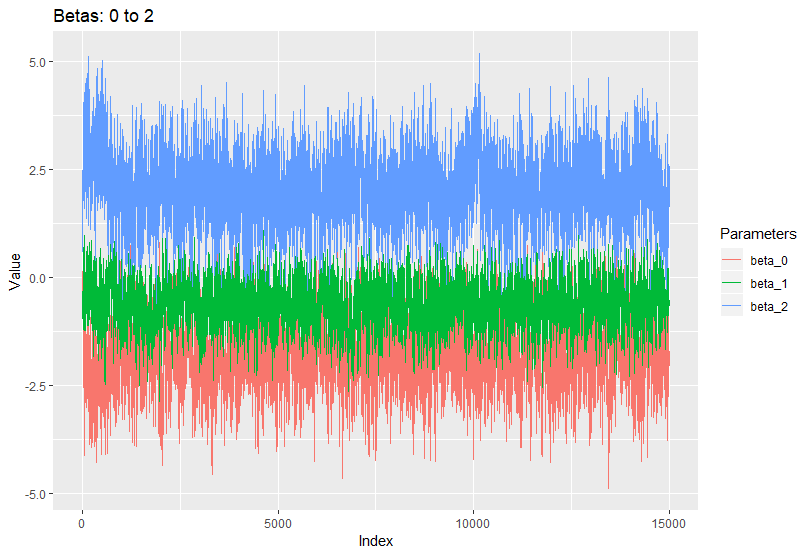
\includegraphics[width=\textwidth]{Cap3/T1Chain}
        \caption{Trazas de la cadena}
        \label{img:GibbsChain}
    \end{subfigure}
	\\
    \centering
    \begin{subfigure}[b]{0.45\textwidth}
        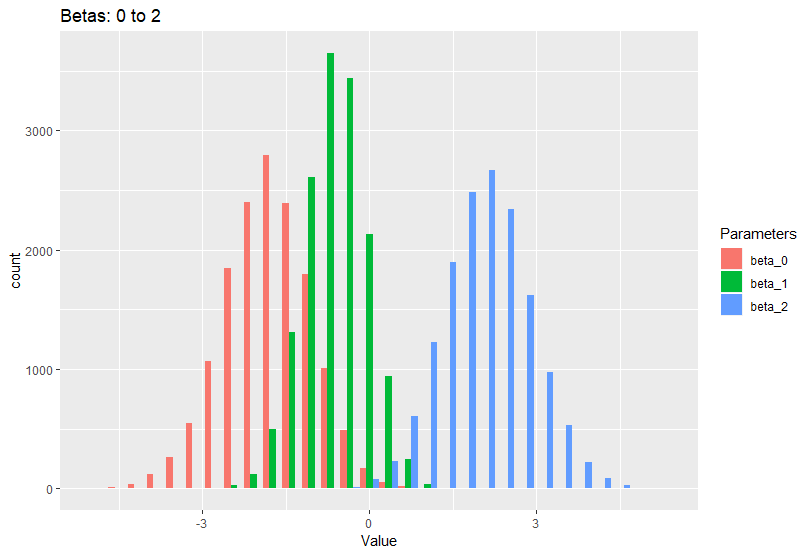
\includegraphics[width=\textwidth]{Cap3/T1Hist}
        \caption{Histogramas}
        \label{img:GibbsHist}
    \end{subfigure}
    \caption{Muestro Gibbs para el ejemplo 1 (sección \ref{sec:T1})}\label{fig:GibbsSamplerSimulado}
\end{figure}
La imagen \ref{img:MedErg} presenta la media ergódica de todos los parámetros que se empiezan a estabilizar conforme avanzan el número de iteraciones del algoritmo. En \ref{img:GibbsChain}, se grafican las trazas de los primeros 3 parámetros ($\beta_0$, $\beta_1$ y $\beta_2$) y en \ref{img:GibbsHist} sus correspondientes histogramas.\footnote{Solamente se muestran los primeros tres parámetros (de cinco) para evitar tener gráficos muy saturados.} Se observa como los primeros valores de los parámetros aún no se estabilizan del todo y sus medias fluctúan, asimismo, se puede observar claramente, como los histogramas tienen formas similares a la de una distribución normal; este hecho se esclarecerá en la sección \ref{sec:AlbertChib}. 

\subsubsection*{Mejoras a las cadenas}
Como se observó en las imágenes previas, el muestreador de Gibbs aunque útil, no es infalible.\footnote{En el sentido que no genera una muestra de v.a.i.i.d.} No obstante, las cadenas pueden ser mejoradas de dos formas sencillas. La primera se conoce como \textit{burn-in} y consiste en eliminar los primeros $(k^*)$-esimos valores simulados de la cadena. Esto dado que el valor inicial $\theta\iter{0}$ es fijado por el estadístico, por lo que en ocasiones el algoritmo tiene que explorar una región extensa de posibles valores de $\theta$ para converger. Por lo tanto, si se busca una muestra de distribución posterior $\pi(\theta)$ los primeros valores pueden ser descartados. El corte $0<k^*<\nsim$ es decidido de forma subjetiva una vez que se explora la cadena entera, ya sea por resúmenes numéricos o por representaciones gráficas. El segundo método es conocido como adelgazamiento (\textit{thinning}) y consiste en tomar cada $(\kthin)$-ésimo valor de la cadena para reducir (más no desaparecer) la dependencia entre los parámetros. Esto ocurre porque las cadenas de Markov, sobre las que depende el muestreador de Gibbs, son generadas de forma secuencial con base en el valor actual actual de la cadena (propiedad markoviana). Por lo tanto, los valores simulados están altamente correlacionados. Sin embargo, estos sencillos pasos para mejorar las cadenas logran mejorar las muestras y ya se encuentran implementados en el paquete.

Una vez estudiadas las herramientas que proporciona la estadística bayesiana, se observa como se comienza a combinar el componente teórico con el componente computacional del modelo haciéndose casi indistinguibles. De la misma forma, se prepara el terreno para terminar de definir el modelo, induciendo así el algoritmo de aprendizaje para los parámetros.

\end{document}


